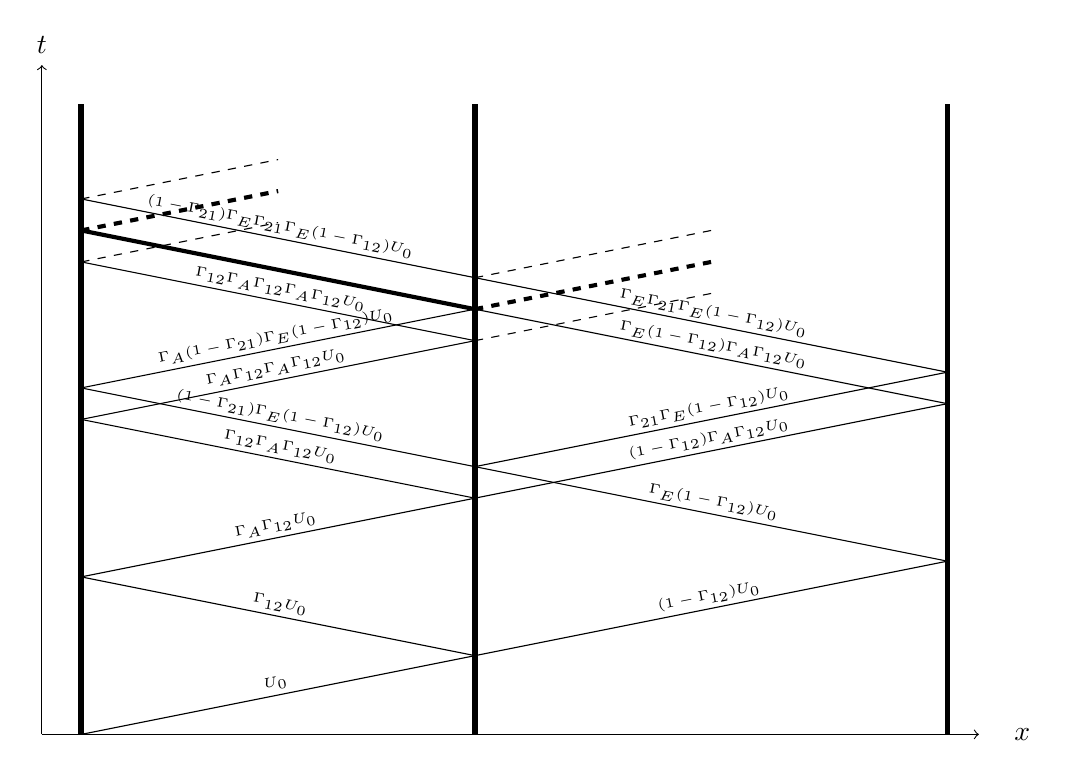
\begin{tikzpicture}
	\draw[line width=2pt] (0,0) -- (0,8);
	\draw[line width=2pt] (11,0) -- (11,8);
	\draw[line width=2pt] (5,0) -- (5,8);
	\draw[->] (-0.5,0) -- node [yshift = 4.5cm]{$t$} (-0.5,8.5);
	\draw[->] (-0.5,0) -- node [xshift = 6.5cm]{$x$} (11.4,0);
	% Linie1
	\draw (0,0) -- node [rotate=11,yshift=0.15cm]{\tiny$U_0$} (5,1);
	\draw (5,1) -- node [rotate=11,yshift=0.15cm]{\tiny$(1-\Gamma_{12})U_0$} (11,1/5*11);
	\draw (11,1/5*11) -- node [rotate=-11,yshift=0.15cm]{\tiny$\Gamma_E(1-\Gamma_{12})U_0$} (5,1/5*11+1/5*6);
	\draw (5,1/5*11+1/5*6) -- node [rotate=-11,yshift=0.15cm]{\tiny$(1-\Gamma_{21})\Gamma_E(1-\Gamma_{12})U_0$} (0,1/5*11*2);
	\draw (0,1/5*11*2) -- node [rotate=11,yshift=0.15cm]{\tiny$\Gamma_A(1-\Gamma_{21})\Gamma_E(1-\Gamma_{12})U_0$} (5,1/5*11*2 + 1);
	\draw[dashed,line width=1.5pt] (5,1/5*11*2 + 1) -- (8,1/5*11*2+1+1/5*3);

	% Linie2
	\draw (5,1) -- node [rotate=-11,yshift=0.15cm]{\tiny$\Gamma_{12}U_0$} (0,2);
	\draw (0,2) -- node [rotate=11,yshift=0.15cm]{\tiny$\Gamma_A\Gamma_{12}U_0$} (5,3);
	\draw (5,3) -- node [rotate=11,yshift=0.15cm]{\tiny$(1-\Gamma_{12})\Gamma_A\Gamma_{12}U_0$} (11,1/5*11+2);
	\draw (11,1/5*11+2) -- node [rotate=-11,yshift=0.15cm]{\tiny$\Gamma_E(1-\Gamma_{12})\Gamma_A\Gamma_{12}U_0$} (5,1/5*11+1/5*6+2);
	\draw[line width=1.5pt] (5,1/5*11+1/5*6+2) -- (0,1/5*11+1/5*6+2+1);
	\draw[dashed,line width=1.5pt] (0,1/5*11*2+2) -- (2.5,1/5*11*2+2+1/2);
	
	%Linie3
	\draw (5,3) -- node [rotate=-11,yshift=0.15cm]{\tiny$\Gamma_{12}\Gamma_A\Gamma_{12}U_0$} (0,4);
	\draw (0,4) -- node [rotate=11,yshift=0.15cm]{\tiny$\Gamma_A\Gamma_{12}\Gamma_A\Gamma_{12}U_0$} (5, 1+4);
	\draw[dashed] (5, 5) -- (8, 1/5*3+5);
%	\draw[dashed] (11, 1/5*6+5) -- (0,1/5*11*2+4);
	
	%Linie4
	\draw (5,5) -- node [rotate=-11,yshift=0.15cm]{\tiny$\Gamma_{12}\Gamma_A\Gamma_{12}\Gamma_A\Gamma_{12}U_0$} (0,6);
	\draw[dashed] (0,6) -- (2.5,1/2+6);
	
	\draw (5,1/5*11*2-1) -- node [rotate=11,yshift=0.15cm]{\tiny$\Gamma_{21}\Gamma_E(1-\Gamma_{12})U_0$} (11,1/5*11*2-1+1/5*6);
	\draw (11,1/5*11*2-1+1/5*6) -- node [rotate=-11,yshift=0.15cm]{\tiny$\Gamma_E\Gamma_{21}\Gamma_E(1-\Gamma_{12})U_0$} (5,1/5*11*2-1+1/5*6*2) -- node [rotate=-11,yshift=0.15cm]{\tiny$(1-\Gamma_{21})\Gamma_E\Gamma_{21}\Gamma_E(1-\Gamma_{12})U_0$} (0,1/5*11*2-1+1/5*6+1/5*11);
	\draw[dashed] (0,1/5*11*2-1+1/5*6+1/5*11) -- (2.5,1/5*11*2-1+1/5*6+1/5*11 + 1/2);
	
	\draw[dashed] (5,1/5*11*2-1+1/5*6*2) -- (8,1/5*11*2-1+1/5*6*2+1/5*3);
%	\draw[dashed] (11,1/5*6+6) -- (8.5,6+1/5*6+1/2);
\end{tikzpicture} \\